


%%%%%%%%%%%%%%%%%%%%%%%%%%%%%%%%%%%%%%%%%%%%
%%%%%%%%%%%%%%%%%%%%%%%%%%%%%%%%%%%%%%%%%%%%

\chapter{Theme 2: Closed-loop Model Checking for Implantable Pacemaker}
\label{ModelChecking}
%There are two categories of device bugs: 
%1) the device may fail to conform to its \emph{specifications}, that is, the prescription of how it should react to certain inputs.  
%2) the device may fail to improve the conditions of the patient as promised, even if it conforms to its specifications. 
%The desired physiological conditions that the closed-loop system should achieve are captured in the \emph{physiological requirements}; for example, for a pacemaker, the heart rate should always be maintained above a certain threshold. 
%
%Bugs in the first category (non-conformance to specification) can be detected via systematic and extensive open-loop testing in which a set of input sequences is fed to the device, and its output is compared with the expected output.
%Bugs in the second category (violation of physiological requirements), on the other hand, require the interaction within the \emph{closed-loop system}, which consists of the device and its environment.
%For instance, the pacemaker and the heart as its environment. 
%In the medical device industry, closed-loop verification of the physiological requirements is mostly performed in terms of clinical trials, in which the actual devices are implanted in human subjects over an extended duration.
%Unfortunately, because of the extremely high cost of clinical trials (several million dollars and spanning several years,~\cite{trialcost}), the amount and variety of human subjects during the clinical trials are limited, which reduces the opportunity to find bugs. 
%Moreover, clinical trials are often conducted at the final design stage. Fixing bugs at this stage is very costly.

Model checking is a technique in which the state space of the model under investigation is automatically and exhaustively explored to identify executions or states that violate specified properties. Violations of the properties are returned by the model checkers as \emph{counter-examples}, which can be used by designers to revise the design. In the application of verification of properties in medical devices like implantable pacemaker, model checking can be used to identify known and unknown mechanisms for inducing hazards. This is extended to checking the heart-pacemaker closed-loop models against physiological hazards (e.g. when the pacemaker provides inappropriate therapy which drives the heart to an unsafe state). 

Due to the curse of dimensionality as models get more complex, and hence the large computational cost, there are usually restrictions on the formalism and the complexity of the models under investigation. Using abstract models of the actual system adds the responsibility of proving the conformance between the abstract model and the real system. Assumptions made during abstractions may also introduce false-positives and/or false-negatives into the model checking results. Back in Chapter 2, we introduced a set of heart models with different abstraction levels, that can be used to cover behaviors of physiological conditions using non-determinism. In Chapter 4, we then modeled a dual chamber pacemaker algorithm using timed-automata without doing abstractions. In this chapter, we use model checker UPPAAL to evaluate the pacemaker model against safety properties under different heart conditions captured by the heart models. Techniques to eliminate false-positives by refining the heart models are also discussed. We will try to answer the following questions:
\begin{figure}[!t]
		\centering
		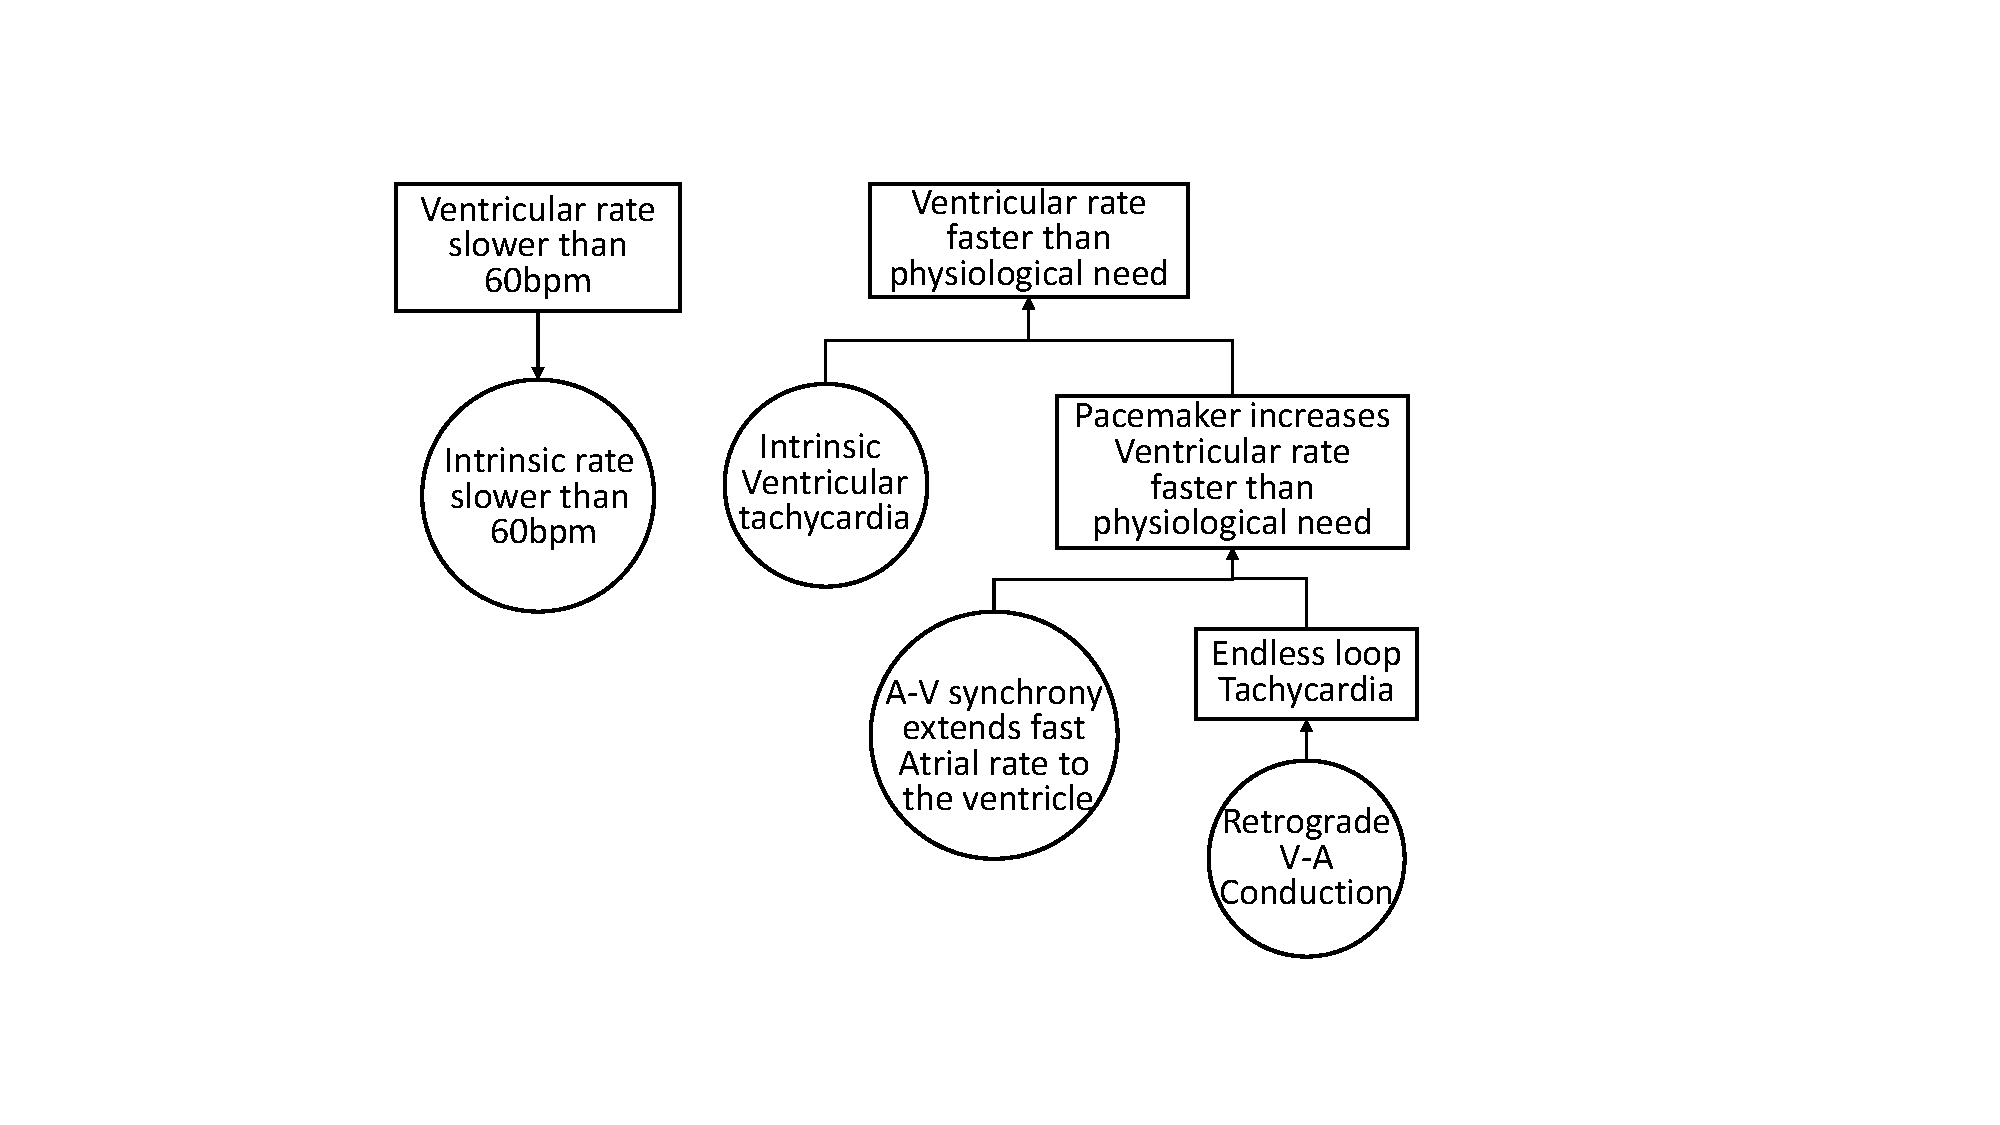
\includegraphics[width=0.8\textwidth]{figs/risk_requirements.pdf}
		\caption{\small Sample Fault Tree Analysis of the physiological conditions leading to the lower rate limit and upper rate limits}
		  %\vspace{-15pt}
		\label{fig:risk_req}
\end{figure}

%            \item What are the effects of adding new features to the software? Can they disrupt the safety properties that the previous device hold?

%In closed-loop model checking, there is only one device model. 
%However there can be a large number of environmental conditions which require different models to represent them. For instance, a heart with atrial flutter has an additional conduction pathway, causing fast atrial rate, that is not present in a healthy heart. The timing and structural differences of different heart conditions should be distinguished in corresponding heart models.
%%\todo[inline]{should we give an example of a heart condition?}
%A set of initial models of the environment can be constructed, but the set is inherently incomplete because of the large number of environment conditions and their combinations. 
%As a result, performing model checking using every model in the set cannot ensure full coverage of the environmental conditions. In the following sections, we will investigate how as we go from basic to more complex requirements, we require more sophisticated approaches to generate and navigate through a variety of environment models. We introduce the concept of an \emph{Abstraction Tree} to systematically encode requirements and choose the appropriate heart models for the requirement. By analyzing the concrete counter-examples we are able to distinguish if the problem is a bug within the device or due to the lack of expressiveness in the environment model. 
\begin{itemize}	
\vspace{-5pt}
	\item How do model checking results fit into the regulation framework?
	\vspace{-5pt}
	\item How do we find the appropriate abstraction level of the environment model for each physiological requirement?
        \vspace{-5pt}
        \item How do we interpret abstract counter-examples returned by model checker?
\end{itemize}
%\section{Testing vs Verification}
%
%\newcommand{\ub}{\bar{u}}
%\newcommand{\yb}{\bar{y}}
%
%\emph{\textbf{Testing}} is a method for checking that a system does indeed obey its specification. 
%In testing, an algorithm will do the following:
%\begin{itemize}
	%\item Initialize the system to some initial state $x_0$ in $X_0$.
	%E.g., for a pacemaker device, this would describe the initial values for the various refractory periods, among other things.
	%\item Generate sequences of input strings $\bar{u}_k$ from some set $A$, in reaction to which the system will produce output strings $\bar{y}_k$,
	%\item A \emph{monitor} logs the output strings and determines whether the pair $(\bar{u}_k,\bar{y}_k)$ satisfies the specification or not.	
%\end{itemize}
%
%Because the set of valid initial states $X_0$ and the set of valid input strings $A$ may be infinite (or simply too large), the test bench must decide on how to intelligently choose a \emph{finite} number of $(x_0,\ub)$.
%They must be chosen such that if the system does not produce wrong behavior with these pairs, then it is unlikely to produce errors under the \emph{full} valid set of pairs, namely, $X_0 \times A$.
%This is the main challenge of testing: how to sample an infinite or large set of behaviors such that it is representative (in the above sense) of the full set of behaviors that $S$ is capable of?
%Another important issue in testing is for how long to test the system: i.e. what should be the length of the $k^{th}$ string $\ub_k$? 
%E.g., if $\ub_k$ has length 1000, the bug might manifest itself on $y_1\ldots y_{1001}$, but not $y_1\ldots y_{1000}$.
%
%Regardless of the testing algorithm, testing remains incomplete, in the sense that short of testing every possible behavior, bugs may lie hidden in the behavior that we did not witness.
%
%\emph{\textbf{Verification}} refers to formal verification.
%It is applicable to finite state systems\footnote{Some infinite-state systems can be formally verified after an abstraction process which essentially produces an equivalent system that has finitely many states.}, 
%and requires formal semantics for the system's operation. 
%Roughly, this means we must have a mathematical unambiguous definition of how the system produces its output.
%A verification algorithm, or \emph{model checker}, will explore the \emph{entire finite state-space} of the system in a systematic manner. 
%Intuitively, if the entire state-space has been explored in all possible ways, and no incorrect behavior has been displayed, then the system is correct. 
%Thus, verification is inherently \emph{complete}: if the model checker determines that the system is correct (under the conditions $A$ and $X_0$), then we can rest assured that is indeed the case.
%Unlike testing, there is no question of whether we missed (didn't run) an initial condition that can display a bug.
%There is also no question of test duration.
%However in practice, some bound on the duration of the verification must be placed to avoid excessively long runs. 
%If the model checker can't determine correctness in that time bound, then the verification is inconclusive.
%
%Verification is computationally expensive and usually more burdensome to setup, but comes with a guarantee on the answer. 
%Testing is computationally cheaper and less burdensome to setup, but the guarantees it provides are significantly weaker.
%Testing, on the other hand, may be the only option for some complex systems that are beyond the capacity of today's model checkers, or which do not possess formal semantics.
%
%In this chapter we cover formal verification of the closed-loop system and address testing in the following chapter.
\section{Risk Analysis for Implantable Pacemaker}
Implantable pacemakers are designed to treat bradycardia by increasing the heart rate with external pacing. Therefore the heart rate should not only be increased to the minimum physiological need, but also should not be increased beyond physiological need. \figref{risk_req} demonstrates two Fault Tree Analysis (FTA) for these two top level hazards. In the remaining chapter we first specify hazards as properties, and use model checking to evaluate whether these hazards have been mitigated by the pacemaker. Then for one of the mitigation algorithm, we examine the mitigation effectiveness and the residue hazard.

\section{Mitigating Top-level Hazards}
The most essential function for the pacemaker is to treat bradycardia by maintaining the ventricular rate above a certain threshold. We define the region where the ventricular rate is slow, as \textsf{unsafe}. The monitor \textsf{PLRI\_test} is designed to measure intervals between ventricular events and is shown in \figref{safety1}. For property
\begin{center}
\textsf{$\varphi_{LRI}=$A[] (PLRI\_test.secV imply PLRI\_test.t$\leq$TLRI)}
\end{center}
we have a closed-loop system  with heart model $H_d$ (described in at the end of Chapter 2): 
$$H_4\| P\| PLRI\_test\models\varphi_{LRI}$$

\begin{figure*}[t]
\centering
%\vspace{-10pt}
		\subfigure[Monitor \textsf{PLRI\_test}] {
				\includegraphics[width=0.5\textwidth]{figs/LRI_test.pdf}
				\label{fig:safety1}
		} 
		\subfigure[Monitor \textsf{PURI\_test}] {	
			\includegraphics[width=0.45\textwidth]{figs/uri_test.pdf}
			\label{fig:uri_test}
		}
		%\vspace{-10pt}
	\caption{(a) Monitor for LRL: Interval between two ventricular events should be less than TLRI, (b) Monitor for URL: Interval between a ventricular event and a VP should be longer than TURI}
\vspace{-10pt}
\end{figure*} 

The pacemaker is not designed to treat tachycardia so it can only pace the heart to increase its rate and cannot slow it down. To mitigate the hazard that the pacemaker may increase the heart rate above physiological need, an Upper Rate Interval (URI) is specified such that the pacemaker can increase the ventricular rate up to this limit. 

\begin{figure}[b]
		\centering
		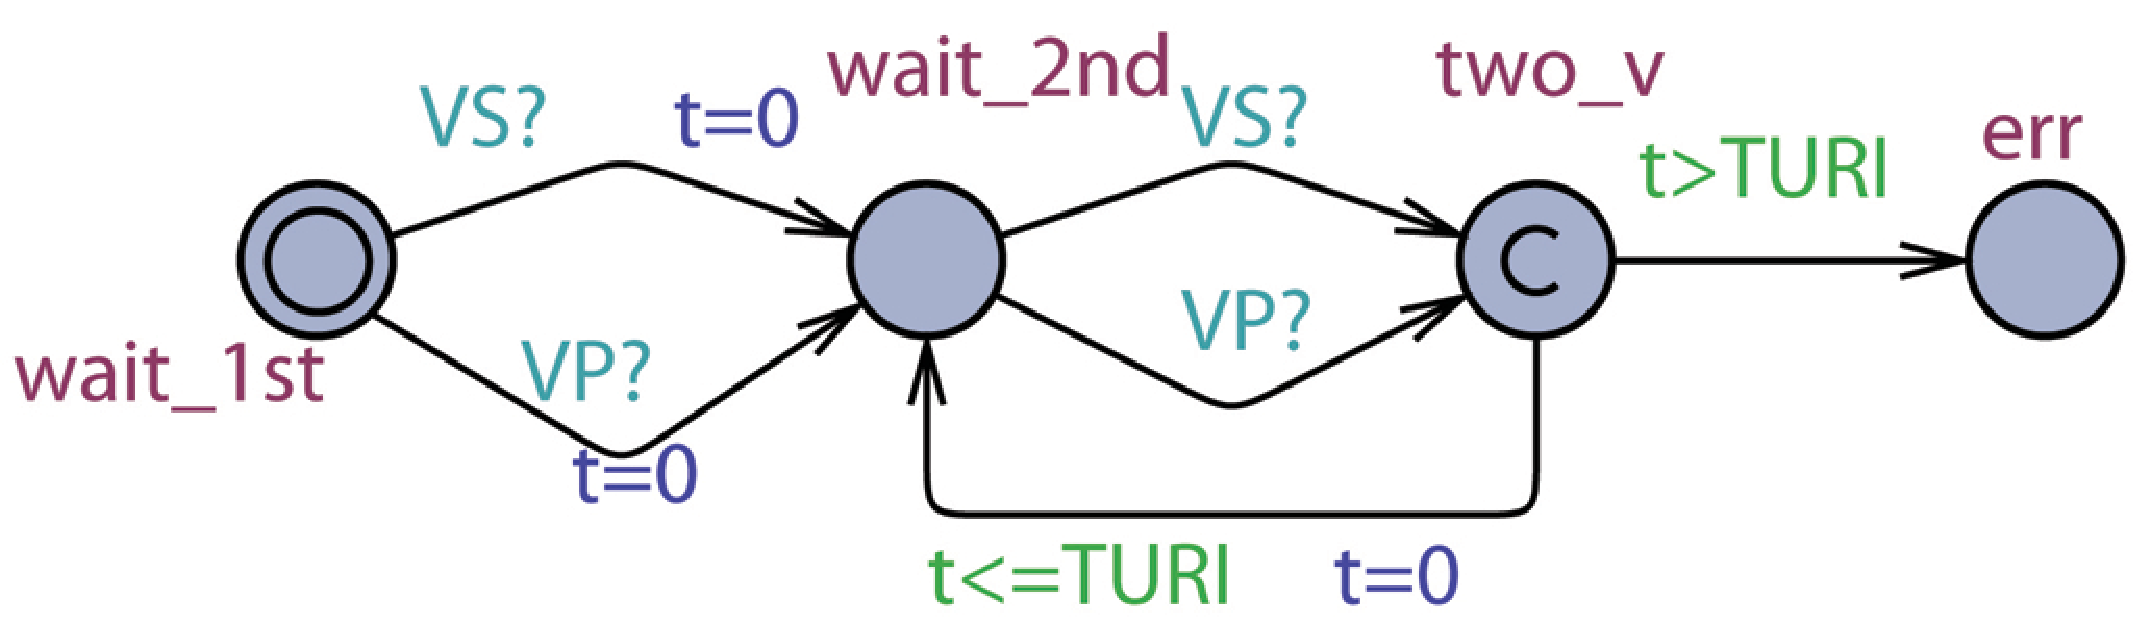
\includegraphics[width=0.4\textwidth]{figs/vv.pdf}
		\caption{\small Monitor \textsf{Pv\_v} for SVT: There exists an endless sequence in which interval between ventricular events is at most TURI}
		  %\vspace{-15pt}
		\label{fig:vv}
\end{figure}
  
We require that a ventricle pace (VP) can only occur at least $TURI$ after a ventricle event (VS, VP). The monitor \textsf{PURI\_test} is shown in \figref{uri_test}. For the property
\begin{center}
$\varphi_{URI}=$\textsf{A[] (PURI\_test.secV imply PURI\_test.t$\geq$TURI)}
\end{center}
we have: $$H_d\| P\| PURI\_test\models \varphi_{URI}$$

\section{Evaluate the Mitigation}
As described in Chapter \ref{Mode_switch}, the mode switch algorithm has been designed to mitigate the hazard that the A-V synchrony function of DDD pacemaker extends fast
atrial rate to the ventricle. It is important to ensure the effectiveness of the algorithm without inducing other top-level hazards. In this section we first show the existence of the hazard in a pacemaker without the mode-switch algorithm. If the algorithm if effective the hazard will not exist after introducing the algorithm.

\subsection{Existence of Pacemaker Mediated Tachycardia during SVT}
The monitor \textsf{Pv\_v} is designed to show existence of PMT during SVT. It goes to the error state if the ventricular rate drops below the Upper Rate Limit (\figref{vv}).  


We specify 
$\varphi_{MS}=E[] (not Pv\_v.err)$\\
which verifies the existence of PMT. The heart model $H_e$ in Fig. \ref{fig:HM_abs} is not suitable for this property since the non-deterministic conduction of component $P_3$ does not capture the blocking property of the AV node, which is the key in PMT. We use a more refined model $H_d$ which has AV node modeled. To identify the PMT scenario, we first set $H_d.N^1.Trest\_min<100$ so that the atrial rate can be high and $H_d.N^2.Trest\_min>TURI$ so that the intrinsic heart rate is less than TURI. The property is first verified on pacemaker without the mode-switch algorithm. We have $H_d\|P\|Pv\_v\models\varphi_{MS}$ and the evidence returned by the model checker illustrates the PMT scenario.

% There are two separate AVI and LRI components for each mode and switches to the corresponding ones when synchronization signals are received. The clock values are kept so that essential intervals are kept. 
\subsection{Verification against fundamental safety properties}
For a pacemaker with the mode switch algorithm: 

$P_2$=\textsf{LRI'$\|$AVI'$\|$URI$\|$PVARP$\|$VRP$\|$INT$\|$CNT$\|$DUR}, 

we verify the same fundamental safety properties on the pacemaker model with mode-switch algorithm. We have:
$$H_d\|P_2\|PURI\_test\models\varphi_{URI}$$
$$H_d\|P_2\|PLRI\_test\not\models\varphi_{LRI}$$
The Upper Rate Limit property still holds, but the Lower Rate Limit property is violated. The counterexample is proved to be valid after checking the trace of more refined heart models. By analyzing the trace we found that when the pacemaker is switching from VDI mode to DDD mode, the responsibility to deliver VP switched from LRI component to AVI component. Since the clock reference is different (Ventricular events in LRI component and Atrial events in AVI component), the clock value for delivering the next VP is not preserved. As a result, if an atrial event which triggered the mode-switch from VDI to DDD happens within [TLRI-TAVI, TLRI) after the last ventricular event, the next ventricular pacing will be delayed by at most TAVI time, which violates the Lower Rate Limit property (\figref{safety}). 
%%\begin{figure}
%%		\centering
%%		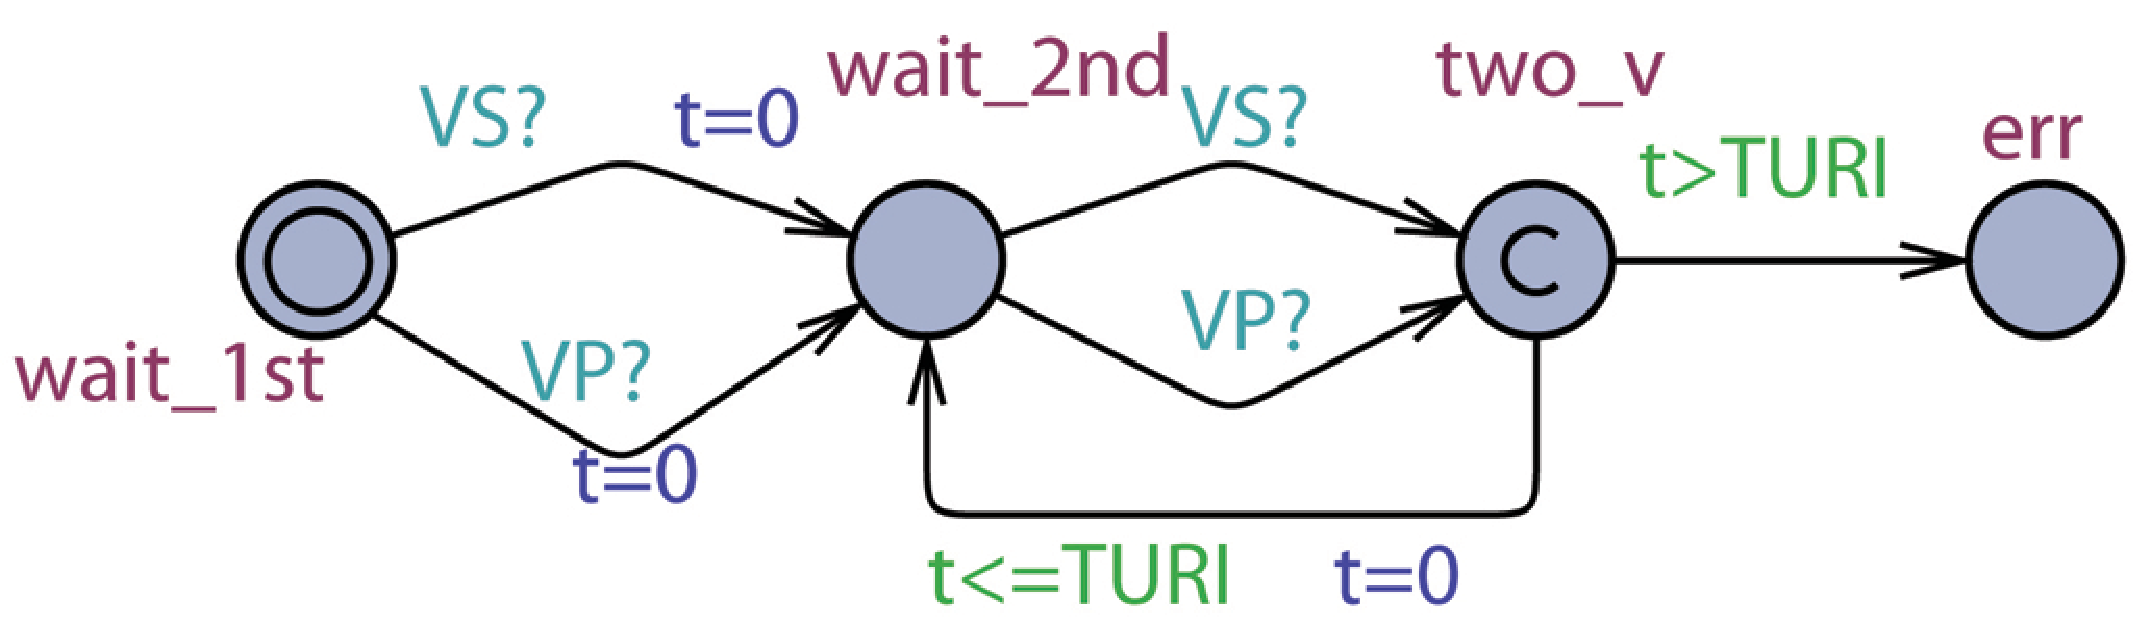
\includegraphics[width=0.4\textwidth]{figs/vv.pdf}
%%		\caption{\small Monitor \textsf{Pv\_v} for SVT: There exists an endless sequence in which interval between ventricular events is at most TURI}
%%		  %\vspace{-15pt}
%%		\label{fig:vv}
%%\end{figure}
\subsection{Verification of the Mode-Switch Algorithm}
After implementing the mode-switch algorithm, we verified the model against the same existence property. We expect the violation of this property, since during VDI mode the ventricular rate of the heart model is less than the Upper Rate Limit and will not trigger ventricular pacing. However, this property is still satisfied, indicating the mode-switch algorithm failed to eliminate the PMT scenario. The evidence trace returned by UPPAAL shows that a subset of atrial events fall into the blanking period after a ventricular event (see \figref{liveness}). As a result, two fast events are reduced to one slow event and mode switch may never happen. This scenario does exist in all our refined heart models, we conclude that the trace is physiologically feasible. The mode-switch algorithm in our pacemaker model can not terminate all PMT behaviors as specified as certain mild PMT events are admissible.
\begin{figure}
\centering
%\vspace{-20pt}
		\subfigure []{
				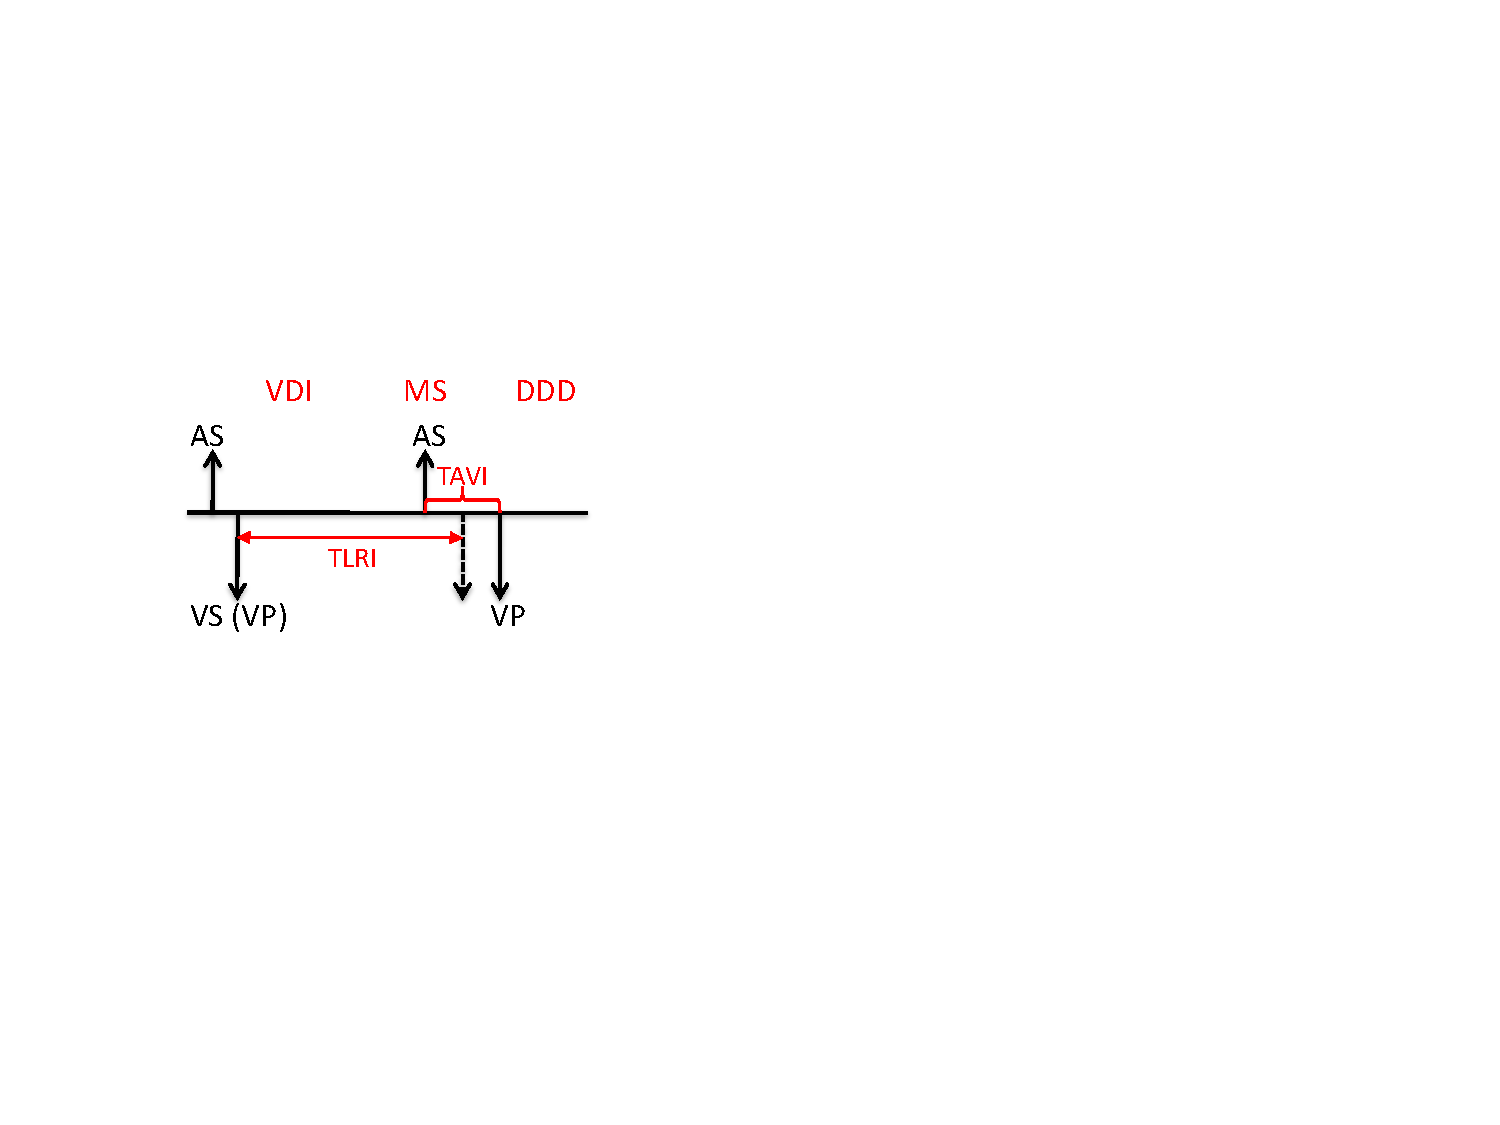
\includegraphics[width=0.4\textwidth]{figs/safety.pdf}
				\label{fig:safety}
		} 
		\subfigure []{	
			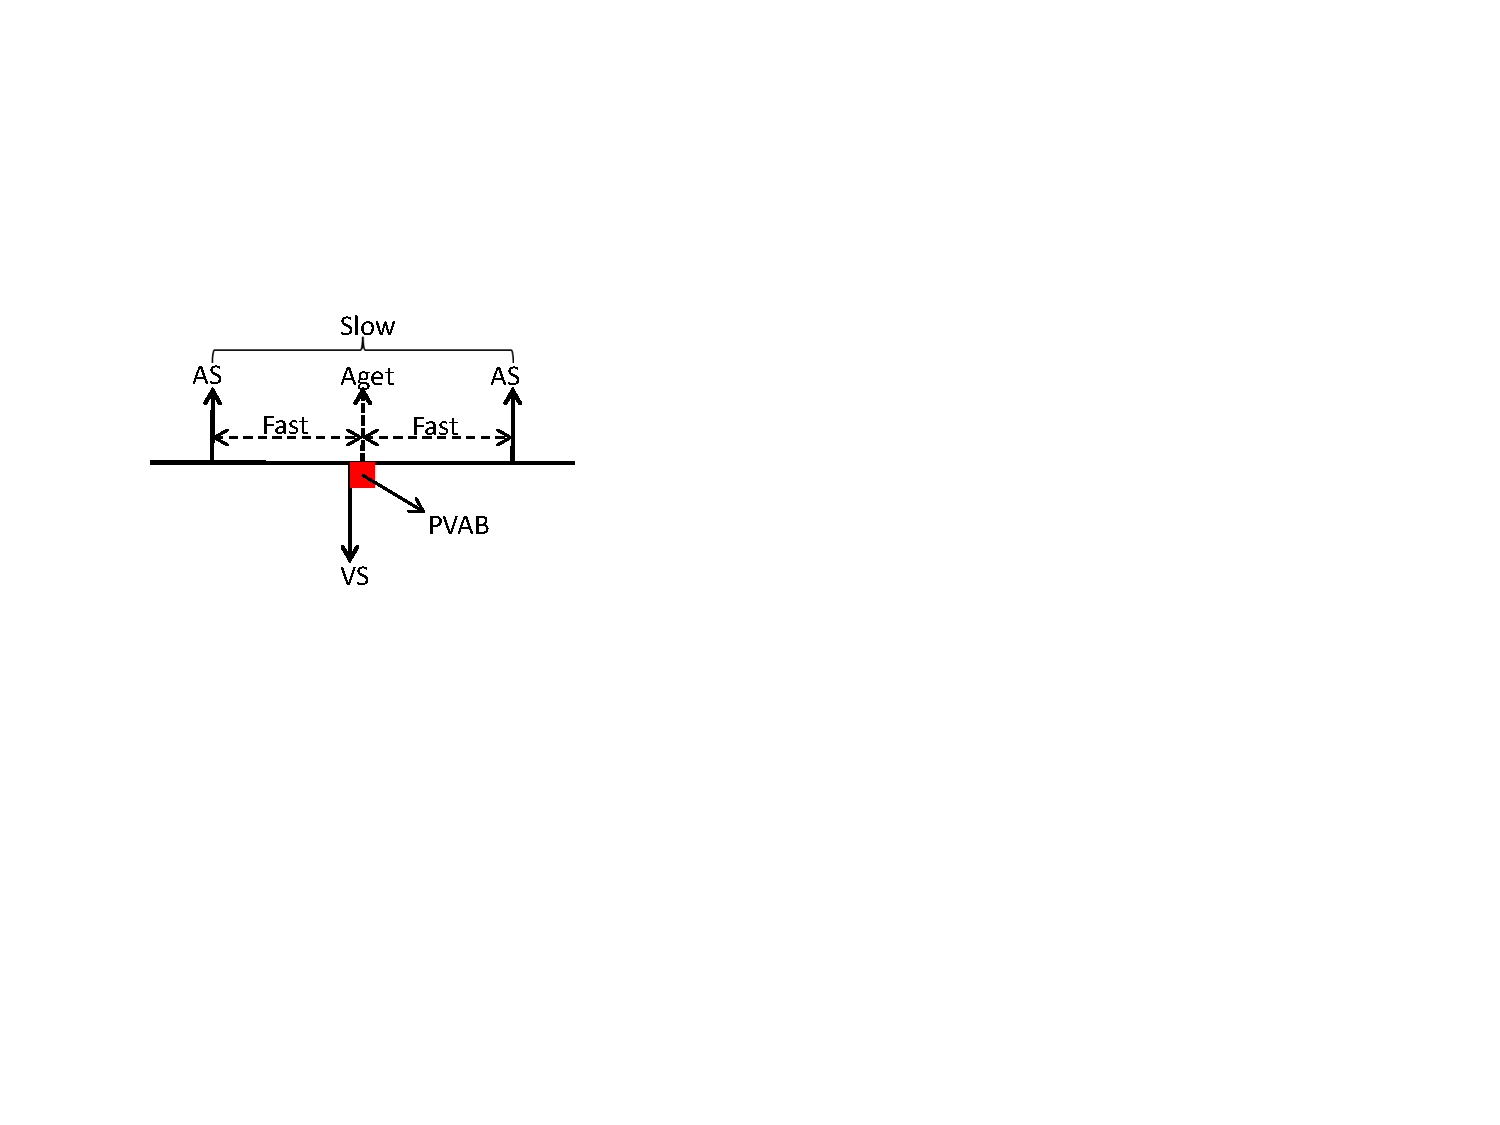
\includegraphics[width=0.4\textwidth]{figs/liveness.pdf}
			\label{fig:liveness}
		}
		\vspace{-10pt}
	\caption{(a) Safety Violation: VP is delayed due to the reset of timer during mode-switch, (b) Correctness Violation: The blocking period may block some atrial events, turning two \emph{Fast} events to one \emph{Slow} event (\cite{TACAS12}})
\vspace{-20pt}
\end{figure} 
\section{Abstraction Tree for Environment Modeling}
In the previous two sections, abstractions and selections of the heart models are performed manually, which require knowledge of both electrophysiology and model checking. 
Counter-examples returned from abstract models can be difficult to interpret by domain experts.
One abstract counter-example could be produced by multiple physiologically valid conditions, which causes ambiguity.
Thus, a rigorous framework is necessary to balance the need to cover a wide range of environmental conditions and the need to provide counter-examples to the physicians within their physiological context. The framework must also allow non-domain experts to perform verification, and establish `hand-off' points where the results of verification can be handed back 
to the experts for interpretation.

In this section, we use a set of domain-specific abstraction rules based on physiological knowledge to ensure the physiological relevance of the behaviors introduced into the abstract models.
The rules are applied to an initial set of physiological models to obtain an abstraction tree, which will be used for closed-loop model checking of the pacemaker. 
A straightforward search procedure is then used to conduct model checking using suitable heart models and return the most concrete and unambiguous counter-examples to the physicians for analysis.
In this framework, physiological knowledge is only needed when constructing the initial model set and when analyzing counter-examples. 
The application of the physiological abstraction rules and the verification procedure can be automated.
The proposed method can potentially be generalized to other domains in which the device operates in a large variety of environmental conditions. More information regarding this research can be found in \cite{regar_tech}.
\subsection*{Step 1: Abstraction Tree construction}
A set of heart models corresponding to different heart conditions are first developed. 
The list can be expanded as new heart conditions are discovered.
Because we start from a set of initial models, and each one may be abstracted using a number of abstraction rules, we have a choice of which rules to apply to which models, and the order in which to apply them. 
Depending on which rule is applied when, we end up with different abstract models.
Thus an \emph{abstraction tree} $T_{HM}$ for the heart is created, as shown in \figref{HM_tree}. 
%Note that applying rules in different order results different abstraction tree. 
%The order used to obtain $HM\_tree$ is based on the domain knowledge that certain heart conditions may have similar behaviors and similar inputs to the pacemaker. 
%This systematic grouping maintains the physiological-relevance of the heart model even at higher abstraction levels, and reduce the necessity to resolve ambiguities at lower abstraction levels when model checking certain requirements.
\begin{figure}[!t]
	\centering
	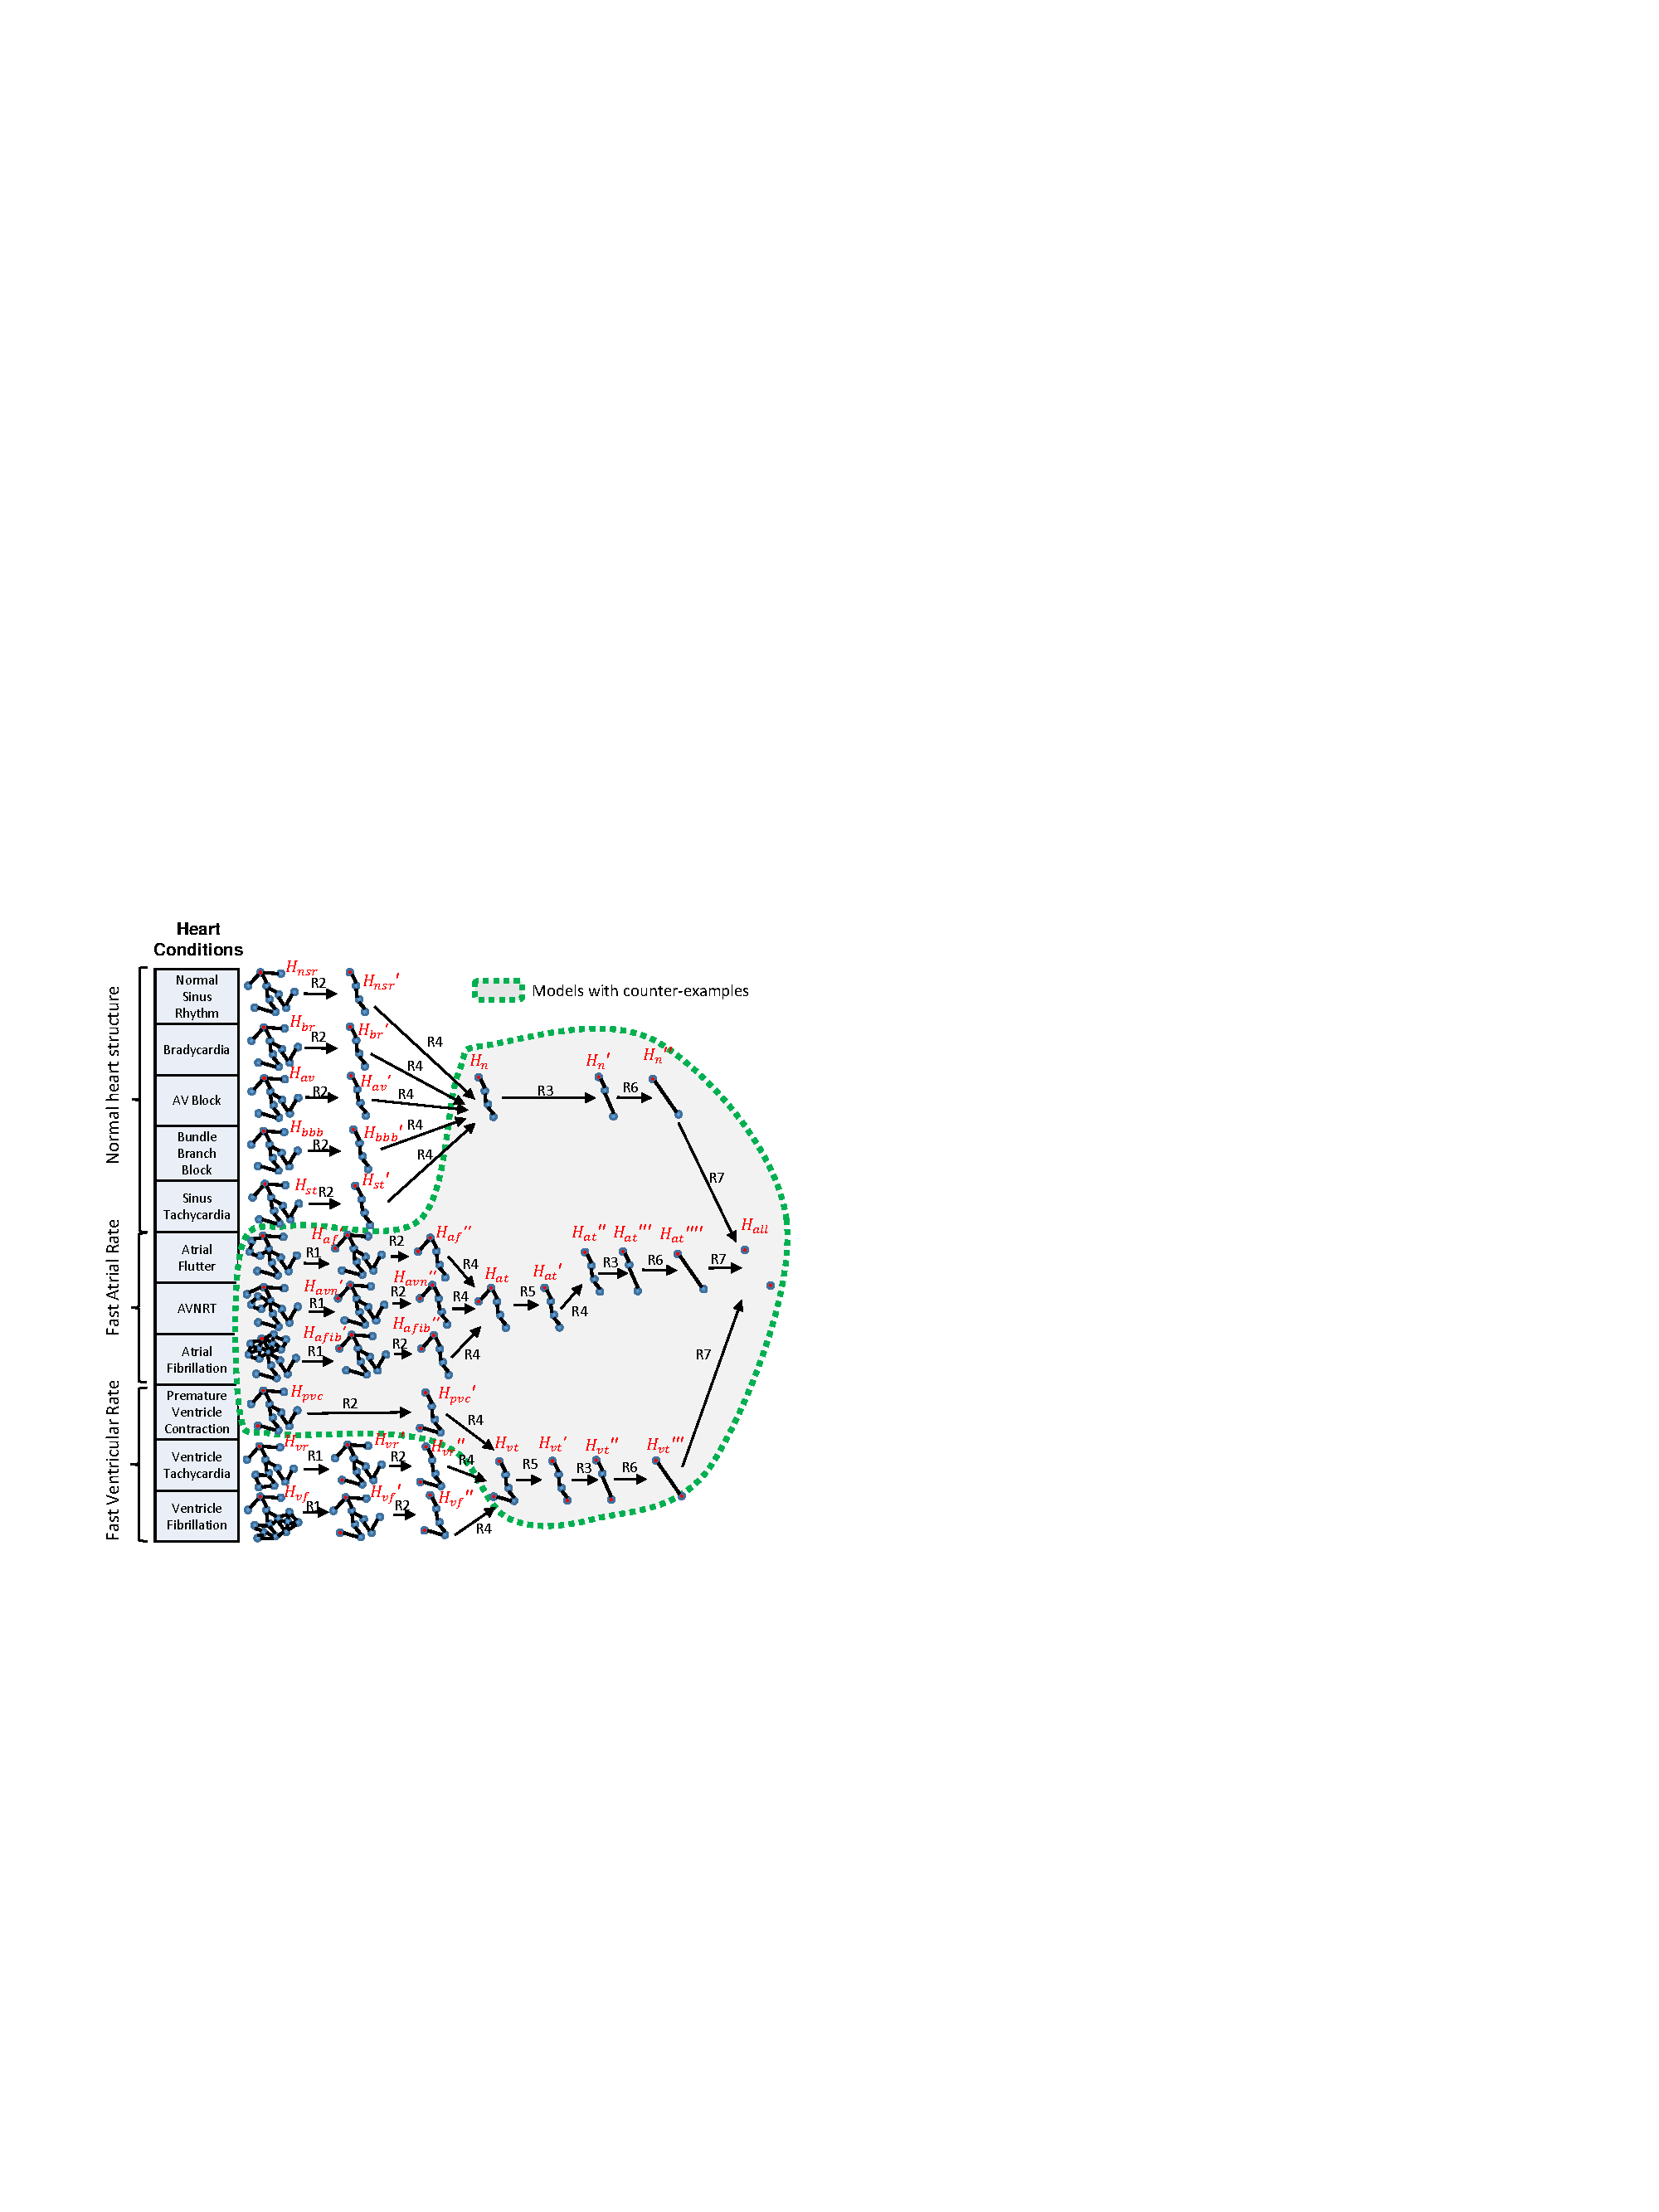
\includegraphics[width=0.85\textwidth]{figs/abs.pdf}
	%\vspace{-5pt}
	\caption{\small Heart Model Abstraction Tree with arrows showing the direction of the abstraction process starting from detailed models of different heart conditions. Model refinement is in the opposite direction.}
	\vspace{-15pt}
	\label{fig:HM_tree}
\end{figure}

\subsection*{Step 2: Requirement encoding}
The following requirement is designed to prevent the pacemaker from pacing too fast: 
``If the intervals between self-activations of the atria are between 300ms to 1000ms (60bpm - 200bpm), the intervals between ventricular paces should be no shorter than 500ms.''
Self-activation of the atria can be expressed using the location and clock of node automaton $N_A$.
The requirement can be formalized using the monitor  $M_{sing}(VP,500,\infty)$:
%\hatodo{mention $N_A$ is the atrium node automaton}
\[Req1: N_A.loc=Rest \land N_A.t\in [300,1000] \Rightarrow \neg M_{sing}.loc==Err\]
%\todo[inline]{some figure captions are all caps, others are not. please use same thing throughout}
%\begin{figure}[!b]
	%\centering
	%\vspace{-10pt}
	%\includegraphics[width=0.5\textwidth]{figs/abs_sim.pdf}
%
	%\caption{\small Abstraction Rule Application Example}
%\vspace{-10pt}
	%\label{fig:abs_exam}
%\end{figure}
 \subsection*{Step 3: Choosing appropriate heart models for the requirement}
To verify the closed-loop system with pacemaker model $PM$ and abstraction tree $T_{HM}$ (\figref{HM_tree}) against requirement $Req1$, the most abstract appropriate models are selected from the tree. 
The single event monitor $M_{sing}$ from \figref{monitor}(a) with variables $Var(M_{sing})=\{M_{sing}.t,M_{sing}.loc\}$ is used for this requirement. Model checking is performed on the closed-loop system including the heart model $M_H$, the pacemaker model $M_P$, and the monitor $M$. The requirement $\varphi_P$ can be then represented with TCTL formula:
\begin{center}
 \textsf{A[] (not M.Err)}
\end{center}
The variables in the requirement are:
$$Var(Req1)=\{N_A.t,N_A.loc,M_{sing}.loc\}$$
\begin{figure}[b]
		\centering
		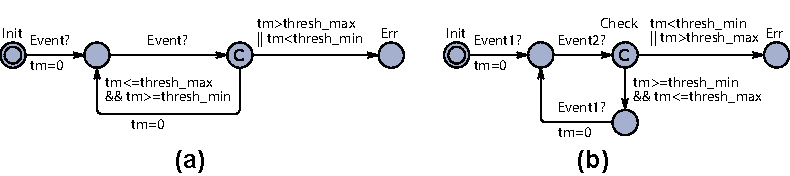
\includegraphics[width=0.8\textwidth]{figs/monitor.pdf}
		%\vspace{-5pt}
		\caption{\small (a) $M_{sing}$ for single event; (b) $M_{doub}$ for two events}
		  \vspace{-10pt}
		\label{fig:monitor}
\end{figure}

At the root of the tree $H_{all}$, we have $\{N_A.t,N_A.loc\} \not \subset Var(H_{all})\cup Var(M_{sing})$. 
So $H_{all}$ is not appropriate for $Req1$. 
All the children of $H_{all}$: $H_n'',H_{at}'''',H_{vt}'''$ are appropriate for $Req1$,
%we have $Var(Req1)\cup Var(M_{sing})\subset Var(H_n'')=Var(H_{at}'''')=Var(H_{vt}''')$, 
thus these three heart models are output as the most abstract models that are appropriate for $Req1$.
\begin{figure}[!t]
	\centering
	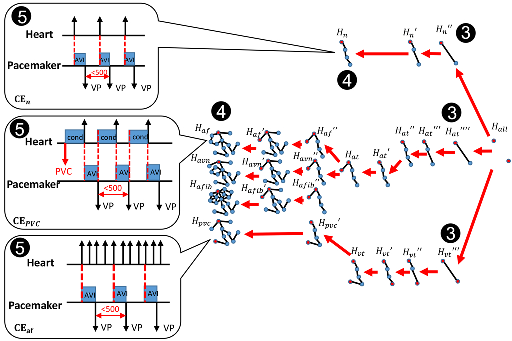
\includegraphics[width=0.8\textwidth]{figs/abs_rev.pdf}
	%\vspace{-5pt}
	\caption{\small Model refinement: Finding the most concrete counter-examples using the abstraction tree}
	\vspace{-10pt}
	\label{fig:CE}
\end{figure}
	\vspace{-10pt}
\subsection*{Step 4: Return the most concrete counter-examples}
After the appropriate models for $Req1$ are selected, we have the initial set
$HM=\{H_n'',H_{at}'''',H_{vt}'''\}$.
By model checking on all three initial models in UPPAAL we have: 
$$H_n''||PM\not\models Req1;\; H_{at}''''||PM\not\models Req1;\; H_{vt}'''||PM\not\models Req1$$
%$$[1,[]]=ModelChecking(H_n'',PM,Req1)$$
 %$$[0,CE_1]=ModelChecking(H_{at}'''',PM,Req1)$$
%$$[0,CE_2]=ModelChecking(H_{vt}''',PM,Req1)$$
%\hatodoin{In the following text you use $CE_{at}$, etc. It's  best to use the letter subscripts in the above equations as well, so it's clear which cex comes from which heart model.}
%For the two heart models $H_{at}'''',H_{vt}'''$ in which the requirement is violated, the algorithm keeps going down the abstraction tree, and upon termination counter-examples are returned for the following heart models
The abstraction tree is then further explored. The heart models with counter-examples are illustrated in \figref{CE}, and the most refined heart models with counter-examples are: $H_{n};H_{pvc};H_{af};H_{avn};H_{afib}$.
%$$[0,CE_{at}]=ModelChecking(H_{at},PM,Req1)$$
%$$[0,CE_{pvc}]=ModelChecking(H_{pvc},PM,Req1)$$
%$$[0,CE_{af}]=ModelChecking(H_{af},PM,Req1)$$
%$$[0,CE_{avn}]=ModelChecking(H_{avn},PM,Req1)$$
%$$[0,CE_{afib}]=ModelChecking(H_{afib},PM,Req1)$$

%\begin{figure}[!t]
		%\centering
		%\includegraphics[width=0.9\textwidth]{figs/case.pdf}
		%%\vspace{-5pt}
		%\caption{\small Counter-examples}
		  %\vspace{-10pt}
		%\label{fig:CE}
%\end{figure}
	\vspace{-10pt}
\subsection*{Step 5: Analysis of the counter-examples}
The counter-examples are then shared with physicians for analysis. In \figref{CE} we highlight three counter-examples. In the first counter-example, the intrinsic heart signals over time with up arrows as atrial activations and down arrows as ventricular activations. The signal for the second counter-example shows the pacemaker outputs with up arrows as atrial pacing and down arrows as ventricular pacing.%We only show the activations of the atrial node and ventricle pacing. 

Counter-example $CE_{n}$ is returned by $H_n$ and none of its children models violate the requirement. By careful analysis we found that $CE_{n}$ features the combination of fast intrinsic atrial rate and prolonged A-V conduction delay, which is the combination of heart conditions $H_{st}$ and $H_{av}$. This scenario shows that the abstraction rules can introduce physiological heart conditions that were not explicitly modeled in the initial model set. The pacemaker improved the open-loop heart condition by pacing the ventricles $AVI$ after each atrial event, which is a correct operation of the pacemaker despite the requirement violation. 
%\hatodo{is it TAVI or AVI like in the previous seciton?}

%\hatodoin{Do you mean that $CE_{at}$ is not a bug? Does this mean that the requirement may be violated in ways that are not dangerous?}
Counter-example $CE_{pvc}$ has a very similar execution to $CE_{n}$. However, the activations of the atrial node are triggered by retrograde conduction from ventricle to the atrium initialized by ventricular paces (marker \textsf{cond}). The atrial activations trigger another ventricular pace after $AVI$, which will trigger another retrograde conduction. In this case, the heart rate is inappropriately high, which corresponds to a dangerous closed-loop behavior referred to as \emph{Endless Loop Tachycardia}.

In counter-example $CE_{af}$, the atrial rate is very high, which is also a sub-optimal but not dangerous heart condition. 
However, the ventricular rate can stay normal due to the blocking property of the AV node. 
Despite the filters in the pacemaker, the pacemaker still paces the ventricle for every 3 atrial activations, which extends fast atrial rate to more dangerous fast ventricular rate. 
%\hatodoin{Not very clear..do you mean that the intrinsoc centricular rate is fine because of AV filtering, but the PM is accelarating it?}
This scenario is referred to as Atrial Tachycardia Response of a pacemaker. 

From the analysis, pacemaker operations in $CE_{pvc}$ and $CE_{af}$ must be revised. However, the revision should not affect the behavior in $CE_{n}$. This example demonstrates that counter-examples from refined models provide more physiological context of the requirement violations, and distinguish the physiological conditions that can trigger the violations. The information is helpful for debugging and improving the algorithm. The physicians can also improve the physiological requirement so that these heart conditions can be then considered case by case.\\

\noindent\textbf{Discussion:}\\
Model checking is not widely use in industry, in part, due to scalability issues and also because domain expertise must be a skill possessed by the verification engineer. However, with rigorous abstraction of the system and its environment, model checking can be used to identify 
known and even unknown mechanisms to induce hazards. In this chapter, we use a model of a dual chamber pacemaker as an example to demonstrate the use of model checking during risk analysis. During the process we identified the need to refine the heart models to eliminate false-positives introduced during the abstraction, and demonstrated the difficulty to do so manually. The abstraction tree approach is then proposed to reduce the effort needed for both the developers and the domain experts, which makes model checking a viable approach for providing safety and effectiveness evidence. 
